%%
%\listfiles
%\documentclass[%
% reprint,%
%secnumarabic,%
% amssymb, amsmath,%
% aip,cha,%
%groupedaddress,%
%frontmatterverbose,
%]{revtex4-1}
\documentclass[twocolumn,amsmath,amssymb,showpacs,pre,nofootinbib,superscriptaddress]{revtex4-1} %,preprint,jcp

\bibstyle{apsrev}
%\usepackage{docs}%
\usepackage{bm}%
\usepackage{graphicx}
%\usepackage{subcaption}
\usepackage{tikz}
\usepackage{ulem}
\usepackage{color}
\usepackage{xcolor}
\usepackage{physics}
\usepackage[colorlinks=true,linkcolor=blue]{hyperref}%
%\nofiles
\expandafter\ifx\csname package@font\endcsname\relax\else
 \expandafter\expandafter
 \expandafter\usepackage
 \expandafter\expandafter
 \expandafter{\csname package@font\endcsname}%
\fi
\hyphenation{title}
\newcommand{\figloc}[1]{Figures/#1}

\begin{document}

\definecolor{pyblue}{HTML}{1F77B4}
\definecolor{pyorange}{HTML}{FF7F0C}
\definecolor{pygreen}{HTML}{2CA02C}
\definecolor{pyred}{HTML}{D62728}

\title{Droplet coalescence assisted with surface tension gardients}

\author{S. Zitz}
\email{zitz@ruc.dk}
 \affiliation{IMFUFA, Department of Science and Environment,\\ Roskilde University, Postbox 260, DK-4000 Roskilde, Denmark}%
 \affiliation{Department of Chemical and Biological Engineering, Friedrich-Alexander-Universit\"at Erlangen-N\"urnberg, F\"{u}rther Stra{\ss}e 248, 90429 N\"{u}rnberg, Germany}%
 \author{T. Richter}%
%\email{t.richter@fz-juelich.de}
 \affiliation{Helmholtz Institute Erlangen-N\"urnberg for Renewable Energy,\\
  Forschungszentrum J\"ulich,
  F\"urther Strasse 248, 90429 N\"urnberg, Germany}%
  \affiliation{Department of Physics, Friedrich-Alexander-Universität Erlangen-Nürnberg, \\Fürther Straße 248, 90429 Nürnberg, Germany}%
 \author{K. Missios}%
%\email{missios@ruc.dk}
 \affiliation{IMFUFA, Department of Science and Environment,\\ Roskilde University, Postbox 260, DK-4000 Roskilde, Denmark}%
%\author{H. Scheufler}%
%\email{henning.scheufler@dlr.de}
%\affiliation{DLR German Aerospace Center,\\ Institute of Space Systems, 28359 Bremen, Germany}%
 \author{J. P. Roenby}%
\email{johan@ruc.dk}
 \affiliation{IMFUFA, Department of Science and Environment,\\ Roskilde University, Postbox 260, DK-4000 Roskilde, Denmark}%
\date{\today}

\begin{abstract}
We numerically study the coalescence dynamics of two sessile droplets.
The droplets are placed on top of a rigid substrate with a contact angle of $\theta_{eq.} = \pi/9$. 
% Due to minimization of surface energy, the two droplets are likely to coalescence into a single droplet.
Having a highly wettable substrate ($\theta_{eq} \ll \pi/2$) theory predicts that the bridge height ($h_0$) scales according to $h_0(t) \propto t^{2/3}.$
This behavior can be altered with e.g. surface tension gradients ($\partial\gamma(x) \neq 0$). 
Which appear for example using heating devices, surfactants or having different but miscible liquids.
Instead of coalescence, these gradients can lead to a stable two droplet state. 
In this work, we focus on the influence of the surface tension gradient in the thin film regime. 
We therefore introduce a disjoining pressure and couple it to the surface tension gradient.
Showing that coalescence can be suppressed and retrieving the $2/3$ powerlaw for a vanishing gradient.
Between those two extrema we find intermediate bridge growth and asymmetric coalescence.
\end{abstract}

\maketitle

\newcommand{\ts}{\textsuperscript}

\section{Introduction}\label{sec:intro}
The coalescence or non-coalescens of liquid droplets is an interesting problem to study. 
Both scenarios can be observed in many instances of our every day life and in various industrial processes.
Coalescence of sessile droplets happens, for example, when vapor condenses on the lid of a pot.
Starting with the nucleation of small droplets, which quickly assemble in larger drops either naturally~\cite{PhysRevA.43.1906} or due to artifical factors such as surface structure~\cite{C1SM06219K}. 
Condensation and coarsening can effectively be used in so-called fog harvesting devices, where ambient water vapor becomes an effective source for liquid water~\cite{zhang2015inkjet, shi2018fog}.
Apart from fog harvesting, coalescence or rather the control of it plays an important part in inkjet printing and printable electronics~\cite{jo2009evaluation, singh2010inkjet, Kim_2005, Luechinger_2008}.
But also in various microfluidic devices for mixing purposes at low Reynolds numbers coalescence of droplets serves as an effective technique~\cite{https://doi.org/10.1002/pen.760352206, doi:10.1063/1.858199}. 

On the other hand, there are many applications that require droplets not to coalesce.
In hot summer days a fine water spray can help the body to cool down.
Single, small droplets advect the heat from the body and transfer it into the surroundings~\cite{kim2007spray}.
Cooling hot, e.g. near the boiling point, structures is another issue~\cite{JIA2003829}.
Apart from cooling, emulsions are an illustrative example of systems where droplets should not coalesce.
Thinking about Mayonnaise where due to vigorously stirring the oil breaks up in small droplets that mix with the water of the egg yolk.
Proteins and additions like mustard stabilize this state and keep the oil from coalescing~\cite{harrison1985factors, DEPREE2001157}.

Independent of these examples, droplet coalescence has attracted much attention in the past two decades, see refs.~\cite{eggers_lister_stone_1999, duchemin_eggers_josserand_2003, PhysRevLett.95.164503, PhysRevLett.106.114501, doi:10.1063/1.4828721}. 
The basic theoretical arguments, with some modifications, hold true for even more complex scenarios such as coalescence of liquid lenses~\cite{PhysRevLett.124.194502} or quasi 2D liquids~\cite{klopp2020self, doi:10.1021/acs.langmuir.0c02139}.
What is common to all studies however is the fact that the equilibrium state is one where the two droplets have coalesced.
Interestingly, this doesn't always apply.
Quite recently, Kern et al. have shown that viscoplasticity can lead to state uncoalesced states~\cite{https://doi.org/10.48550/arxiv.2203.15617}.
What has been known for some time however is that a surface tension gradient influences the coalescence process. 
This has been shown by Karpitschka et al. in experiments with different miscible liquids~\cite{PhysRevLett.109.066103, doi:10.1021/la500459v, karpitschka2014sharp, bruning2018delayed}.
In their work, Karpitschka et al. identify an effective Marangoni flow that stabilizes the two droplet system.

We revisit that problem with numerical simulations.
First, we move to the regime where the droplet become small and disjoining pressure can no longer be neglected.
Second, we address the impact of the surface tensions gradient beyond the reduction to its absolute contrast.
Therefore, asking if the concrete function of $\gamma(x)$ influences the overall dynamic and turn non-coalescing states into coalescing ones.
On the same note we discuss the growth laws of the liquid bridge and address Marangoni dominated coalescence.

This paper is organized as follows:
Starting in the next section, Sec.~\ref{sec:theory}, we discuss the underlying theoretical model.
Introducing the thin film equation with an additional term due to the Marangoni flow and the disjoining pressure $\Pi(h)$. 
Followed by our choice for modelling $\Pi(h)$, which comprises of thickness dependent powerlaw and a wettability component. 
In Sec.~\ref{sec:method} we discuss the numerical method we use to solve the thin film equation.
We show how to construct an addition term to account for the flow induced due to the Marangoni effect.
The results are presented and discussed in Sec.~\ref{sec:results}.
Showing, first, coalescence and non-coalescence with constant and Heaviside like surface tension.
Relaxing the sharp gradient in the second half of the results section.
Finally, conclusions and summary are provided in Sec.~\ref{sec:sum_conclu}. 

\section{Theory}\label{sec:theory}
The theoretical approach we use to study this system is the lubrication approximation~\cite{Reynolds, RevModPhys.69.931, PhysRevE.63.011208}.
Resulting in the thin film equation, which for a singular horizontal dimension reads~\cite{RevModPhys.81.739, RevModPhys.81.1131, THIELE2014399}
\begin{equation}\label{eq:thin_film_simple}
    \partial_t h = \partial_x \left(\frac{h^3}{3\mu}\partial_x p\right),
\end{equation}
where $\frac{h^3}{3\mu}$ is the mobility $m(h)$\footnote{$m(h) = h^3/3\mu$ is true only if one assumes a no-slip velocity boundary condition at $h=0$.}, $h(x,t)$ the thickness of the film, $\mu$ is the liquid's viscosity and $p$ it's pressure.
The pressure in this model accounts for the liquid's surface tension, thus the interface minimization, as well as the for correct fluid substrate behavior (wetting)~\cite{PhysRevE.100.033313}.
We can therefore write the pressure as
\begin{equation}\label{eq:pressure}
    p = -\gamma \partial_x^2 h - \Pi(h),
\end{equation}
where the first term is the Laplacian of the liquid-vapor interface (the thickness) and $\Pi(h)$ is the derivative of an interaction potential that is often referred to as disjoining pressure~\cite{RevModPhys.69.931, RevModPhys.81.739, Peschka9275, PhysRevE.63.011208},
\begin{equation}\label{eq:disjoin}
    \Pi(h) = \kappa(\theta)\left[\left(\frac{h_{\ast}}{h}\right)^n - \left(\frac{h_{\ast}}{h}\right)^m\right].
\end{equation}
The prefactor $\kappa(\theta)\propto \gamma\cos(\theta)$ encodes the wettability and with it the contact angle.
It further links the disjoining pressure to the Hamaker constant ($\mathcal{A}$) with~~\cite{PhysRevE.93.013120}
\begin{equation}
    \mathcal{A} = 6\pi h_{\ast}^3\kappa(\theta).    
\end{equation}
Additionally, $h_{\ast}$ defines the thickness of the precursor layer, therefore the thickness where $\Pi(h_{\ast}) = 0$.
For the reminder of this manuscript, we define $h(x,t) \le h_{\ast}$ as a dry spot.
The pair of powers $(n,m)$ need to satisfy $n > m$ and $m > 1$. 
Here we choose $(n,m)$ to be $(9,3)$, which is a widely adopted model that dates back to Schwartz and Eley~\cite{SCHWARTZ1998173, RevModPhys.81.739}.

\begin{figure}
    \centering
    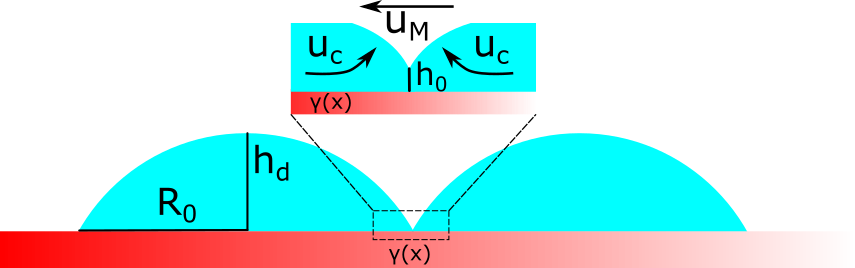
\includegraphics[width=0.48\textwidth]{Figures/setup.png}
    \caption{Schematic setup of the numerical experiment. 
    Two droplets with base radius $R_0$ and maximum height $h_d$ are placed next to each other. 
    They are connected by a liquid bridge with height $h_0$ and subject to a surface tension gradient $\gamma(x)$ .
    The flow has two sizeable contributions, $u_c$ flow due to capillarity and $u_M$ flow due to the Marangoni effect.
    }
    \label{fig:schematics}
\end{figure}
In the presence of a surface tension gradient, Eq.~(\ref{eq:thin_film_simple}) requires an additional term.
The modification is to account for an effective Marangoni flow~\cite{doi:10.1021/la500459v, karpitschka2014sharp, bestehorn20033d, doi:10.1021/la960488a}
\begin{equation}\label{eq:thin_with_marangoni}
    \partial_t h = \partial_x \left(\frac{h^3}{3\mu}\partial_x p + \frac{h^2}{2\mu}\nabla\gamma\right).
\end{equation}
Naturally in case of $\partial_x\gamma = 0$ we retrieve Eq.~(\ref{eq:thin_film_simple}).
These gradients appear due to non-homogenized surfactant concentrations or space resolved heating profiles, e.g. with lasers~\cite{doi:10.1021/la960488a, NIKOLOV2002325, bruning2018delayed, wedershoven2014infrared}.
From an experimental point of view, it could be challenging to precisely control these gradients.
Given the fact that other flow contributions such as heat transport and therefore evaporation should be taken into account as well.
Leaving aside the general treatment of arbitrary surface tension gradients in experiments, a first step would be to introduce a sharp gradient.
First Riegler and Lazar and later Karpitschka et al. have shown that a straightforward realization of a sharp gradient can be achieved with two different but miscible liquids~\cite{doi:10.1021/la800630w, karpitschka2014sharp, doi:10.1021/la500459v}. 

Bringing surface curvature, surface energy gradients and viscous dissipation into balance at a quasi stationary state the film thickness can be approximate with
\begin{equation}
    \partial_x^3 h = 3 \frac{Ca}{h^2} - 3\partial_x\gamma 
\end{equation}
Emerging from that droplet mixture is a surface velocity $u_s$~\cite{PhysRevLett.109.066103}
\begin{equation}\label{eq:Karpitschka_vel}
    u_s = u|_{z=h} = \frac{3v_N}{2} + h\frac{\partial_x\gamma}{4\mu},
\end{equation}
where $v_N$ is the velocity of the neck moving towards higher surface tension.

\section{Method}\label{sec:method}
The method we are using is a numerical one that iteratively solves Eq.~(\ref{eq:thin_with_marangoni}).
Instead, of solving the differential equation directly, see refs.~\cite{PhysRevE.63.011208, PhysRevLett.119.204501}, we use a recently developed lattice Boltzmann method for thin film flows~\cite{PhysRevE.100.033313, PhysRevE.104.034801}.
This approach is based on the evolution of discrete probability density functions ($f_i$) where
\begin{equation}\label{eq:LBE}
    \begin{split}
        &f_i(x+c^{(i)}\Delta t,t+\Delta t) = \\
        &\left(1 - \frac{\Delta t}{\tau}\right) f_i(x,t) + \frac{\Delta t}{\tau} f_i^{(eq)}(x,t) + w_i \frac{\Delta t}{c_s^2} c^{(i)} F,
    \end{split}
\end{equation}
with $F$ being the total forces acting on the fluid.
We adopt the standard D1Q3 (one-dimensional) scheme with $3$ lattice velocities, given by
\begin{equation}\label{eq:speeds}
c^{(i)}  = [0, c, -c], \quad i = 0, 1, 2,
\end{equation}
where the lattice speeds $c=\frac{\Delta x}{\Delta t}$, with weights
\begin{equation}
w_0 = \frac{2}{3},\quad w_{1,2} = \frac{1}{6},
\end{equation}
and the upper bound for information transport, the speed of sound $c_s^2=\frac{c^2}{3}$.
The equilibrium distribution functions $f_i^{(eq)}$ read~\cite{VANTHANG20107373}:
\begin{gather}
    f_{0}^{eq} = h\left(1-\frac{1}{2c^2}gh - \frac{1}{c^2}u^2\right),\nonumber\\
    f_{1}^{eq} = h\left(\frac{1}{4c^2}gh + \frac{1}{2c}u + \frac{1}{2c^2}u^2\right)\label{eq:equilibria},\\
    f_{2}^{eq} = h\left(\frac{1}{4c^2}gh - \frac{1}{2c}u + \frac{1}{2c^2}u^2\right),\nonumber
\end{gather}
where $g$ is the gravitational acceleration that enforces the hydrostatic pressure condition. 
Given the scale of the problem we neglect gravity and set $g=0$.

The film thickness $h$ and the velocity at the free surface $u$ are moments of the distribution functions $f_i$~\cite{Salmon:1999:0022-2402:503, PhysRevE.65.036309, PhysRevE.104.034801}:
\begin{equation}\label{eq:hydrofields}
    h= \sum_{i=0}^2 f_i \qquad hu = \sum_{i=0}^2 c^{(i)} f_i.
\end{equation}
The force $F$ in (\ref{eq:LBE}) accounts for three terms,
\begin{equation}\label{eq:force}
    F = F_{\text{cap}} + F_{\text{fric}} + F_{\gamma}.  
\end{equation}
First being the effect of the film pressure $p$, Eq.~(\ref{eq:pressure}), 
\begin{equation}\label{eq:capillary_force}
    F_{\text{cap}} = -\frac{1}{\rho_0} h \frac{\partial p}{\partial x},
\end{equation}
($\rho_0$ being the fluid density). 
Viscous friction with the substrate is contained in
\begin{equation}\label{eq:fric_force}
    F_{\text{fric}} = -\nu \alpha_{\delta}(h) u,
\end{equation}
where $\nu=\mu/\rho_0$ is the fluid kinematic viscosity (related to the relaxation time $\tau$ by $\nu = c_s^2\left(\tau-\frac{\Delta}{2}\right)$).
The thickness dependent function $\alpha_{\delta}(h)$ is approximately an inverse mobility $m(h)$,
\begin{equation}\label{eq:fric_alpha}
     \alpha_{\delta}(h) = \frac{6 h}{2h^2 + 6h\delta + 3\delta^2},
\end{equation}
with a slip length $\delta$.
The surface tension gradient requires the addition of another forcing contribution $F_{\gamma}$.
Similarly to ref~\cite{PhysRevE.104.034801} we construct a force term and match it to the last term in Eq.~\ref{eq:thin_with_marangoni}, 
\begin{equation}\label{eq:force_gamma_grad}
    F_{\gamma} = \frac{3}{2}\partial_x\gamma(x),
\end{equation}
where we have assumed that the surface tension only varies along the horizontal dimension.
It can be shown that the system of Eqs. (\ref{eq:LBE}-\ref{eq:force_gamma_grad}) represent a solver for the system
\begin{equation}\label{eq:lubr2eq1surf}
\begin{cases}
\begin{array}{ll}
\partial_t h + \partial_x (h u)  = 0 & \\ 
\partial_t (h u) = -\frac{1}{\rho_0}h\partial_x p -\nu\alpha_{\delta}(h)u + \frac{3}{2}\partial_x\gamma.
\end{array}
\end{cases}
\end{equation}

Performing the limits discussed in ref.~\cite{PhysRevE.100.033313, PhysRevE.104.034801}, for exmaple quasistatic this system is an effective solver for Eq~(\ref{eq:thin_with_marangoni}).
There is however a difference to the model used in refs.~\cite{doi:10.1021/la500459v, karpitschka2014sharp}.
The inclusion of the disjoining pressure allows testing the non-coalescence criteria for smaller scales, well below $1mm$ droplet diameter~\cite{karpitschka2014sharp}.

\section{Results}\label{sec:results}

The first scenario we want to test is the simple case of $\partial_x\gamma(x) = 0$.
Therefore a constant surface tension across the whole domain, which is resembled in Eq.~(\ref{eq:thin_film_simple}).
This case has been studied extensively both in experiments and with theory, see refs.~\cite{eggers_lister_stone_1999, PhysRevLett.95.164503, PhysRevLett.111.144502, duchemin_eggers_josserand_2003}. 
Given a small contact contact angle ($\theta \ll \pi/2$) the connecting liquid bridge $h_0(t)$ should follow the powerlaw 
\begin{equation}\label{eq:bridge_power23}
    h_0(t) \propto t^{2/3},
\end{equation}
which can be motivated by using a pressure balance between inertial pressure
\begin{equation}\label{eq:p_inert}
    p_{\text{i}} \propto \rho\left(\frac{h_0}{t}\right)^2,
\end{equation}
and capillary pressure~\cite{doi:10.1021/la800630w}
\begin{equation}\label{eq:p_cap}
    p_{\text{c}} = \frac{2\gamma}{r} \propto \frac{\gamma}{h_0},
\end{equation}
where we assume that $h_0$ scales similar to $r$ the radius of curvature at the touching region.
In Fig.

\begin{figure}
    \centering
    \includegraphics{}
    \caption{Caption}
    \label{fig:my_label}
\end{figure}

\subsection{Bridge growth}\label{subsec:growth}



\subsection{Flows}\label{subsec:flows}

\subsection{Asymmetry}\label{subsec:skewness}


\section{Summary and Conclusions}\label{sec:sum_conclu}
In this work we have repeated the results found by Karpitschka et al., where two sessile droplets although in contact do not coalesce~\cite{karpitschka2014sharp, doi:10.1021/la500459v}

\begin{acknowledgements}

\end{acknowledgements}
\subsection{Comments Tilman}

\begin{itemize}
    \item May I leave comments here?
    
    \textcolor{pyblue}{Stefan}: You may do!
    
    \item I am member of physics departement not Engenering is that important?
    
    \textcolor{pyblue}{Stefan}: I look it up and change that, if you what is the correct affil you can change it as well.
    
    \item \cite{doi:10.1021/la500459v} states that $\Pi(h)$ is neglectable. Maybe do simulations with and without disjoining pressure, that should be a matter of just commenting that part out. If you are lucky it runs stable without major issues and you can show that in your regime there indeed is a difference taking disjoining pressure into account, however big it turns out to be. 
    
    \textcolor{pyblue}{Stefan}: It will not work.
    There is an interface and ``dry`` spots, dry spots can only be done with disjoining pressure.
    I tested this some time ago for some other reason.
    
    My idea is to work out the modified equation with the inclusion of the disjoining pressure.
    But feel free to work on it if you find it interesting.
    
    Theory $>$ Simulation/Experiments!
    
    \item Again \cite{doi:10.1021/la500459v}. In their experiment the surface tension gradient is induced by different liquids. In Figure 2 3b) you see the droplets in the non-coalesence case move thus the surface tension profile moves to. That may be worth to take into account.
    
    \textcolor{pyblue}{Stefan}: Yeah I know.
    The PRL~\cite{PhysRevLett.109.066103} kind of explains why, see Eqs.~(1,2,3).
\end{itemize}

%\input{|python your_script.py}

%\appendix
%\section{}\label{app:one}

\bibliography{Ref}

\end{document}